\section{Web component}
\label{sec:chapter_tecnologie_abilitanti_webcomp_poly}

Al giorno d’oggi le applicazioni web sono molto complesse: è fondamentale trovare il modo corretto di suddividere lo sviluppo dell’applicazione in più componenti non sovrapposte, in modo che il team di sviluppo operi in maniera più efficiente. 
Ogni componente del sistema deve garantire la proprietà di isolamento, per nascondere la propria complessità agli altri componenti.
Un buon isolamento tra componenti rende il software più manutenibile e semplice da sviluppare.
Inizialmente la complessità delle applicazioni web veniva gestita lato server, isolando l’applicazione in più pagine web; questo obbligava l’utente a dover navigare molte pagine sul browser.
Con l’avvento di tecniche come AJAX, che hanno semplificato la realizzazione di single page applications, gli utenti hanno cominciato a fruire di una esperienza d’uso più fluida, simile a quella che si ha con le applicazioni desktop. 
La logica delle applicazione lato client, che spesso è anche più complessa di quella lato server, può essere isolata all’interno di una singola pagina web o documento mediante i web component.
\\
I web component sono un’ insieme di tecnologie prodotte da  Google e approvate dal W3C che consentono la creazione di widget, ovvero elementi html che includono logica di funzionamento e stile, che possono essere importate in documenti o applicazioni web. Da una widget viene separata ogni responsabilità che ha a che fare con altre widget; di conseguenza ogni elemento non dipende dai dettagli implementativi degli altri elementi. Sono possibili dipendenze solo tra le interfacce esposte dalle widget. 
Assegnare le responsabilità in questo modo permette al modello a componenti di soddisfare la proprietà di incapsulamento.
Inoltre la fruibilità di elementi html facilmente integrabili nell’applicazione permette alle componenti di interagire in modo semplice tra loro; in questo modo è soddisfatta anche la proprietà di interoperabilità tra componenti.
Questi web component sono parte del browser, quindi non hanno bisogno di librerie esterne per essere usati, ma basta includerli aggiungendo un tag nella pagina html. 
Una widget è portabile e gode di un elevata riusabilità; inoltre all’interno di una widget è possibile effettuare tutto ciò che è consentito dai linguaggi html, css e JavaScript. 
L’obiettivo principale dei web component è cambiare il modo in cui le applicazioni web vengono create, consentendo agli sviluppatori di estendere il vocabolario HTML creando nuovi elementi HTML riusabili. Questa aggiunta permette agli sviluppatori di interfacciarsi a più alto livello con lo sviluppo di applicazioni web, definibili mediante aggregazione di più componenti.
Quando si parla di web components in verità si parla di quattro tecnologie differenti, le quali insieme forniscono tutti gli strumenti necessari per creare i propri componenti.
Tali tecnologie sono: Custom Elements, Templates, HTML Imports e Shadow DOM. 

La tecnologia \textbf{Custom Element} permette di creare nuovi elementi HTML all’interno del DOM del browser; ogni elemento racchiude logica di funzionamento, stile CSS e un tag HTML necessario per importare l’elemento nelle applicazioni web. 
Nonostante questi elementi facciano parte dei web components, possono essere utilizzati anche come entità separate. Uno dei motivi per cui è stata creata la tecnologia Custom Elements è la possibilità di introdurre le lifecycle callbacks, che consentono di associare specifici comportamenti ad un elemento HTML durante il suo ciclo di vita. Ad esempio è possibile istruire un elemento HTML sul comportamento che deve assumere nel momento in cui viene inserito nel DOM, e su quello che deve assumere quando viene rimosso dal DOM. 
Per registrare un nuovo elemento HTML nel browser si usa il metodo \texttt{Document.registerElement()}, e il nuovo elemento utilizzerà di default l’interfaccia HTMLElement; se invece l’elemento non viene registrato sul browser, userà l’interfaccia HTMLUnknownElement. E’ anche possibile creare un elemento HTML come estensione di un elemento nativo, come \texttt{<button>}; in questo caso però non sarà possibile includere l’estensione nel DOM come elemento a se stante, ma sempre insieme all’elemento nativo che estende; ad esempio l’inclusione sarà \texttt{<button is=”my button”>} e non \texttt{<my-button>} .
I vantaggi apportati dalla tecnologia custom elements sono:
\begin{enumerate}
\item Definizione e creazione di nuovi elementi HTML/DOM.
\item Estendere la logica funzionale di elementi nativi mediante nuovi elementi.
\item Racchiudere tutte le funzionalità di un nuovo elemento in un tag.
\item Estendere le API degli elementi del DOM nativi.
\item Estrema utilità nelle Single Page Applications.
\end{enumerate}
A questo punto verrà mostrato come è possibile creare un nuovo custom element utilizzando ad esempio le classi di JavaScript 6.
Per prima cosa viene definita la classe, la cui struttura è tipicamente la seguente:
\begin{lstlisting}[language=JavaScript]
class MyButton extends HTMLElement {    
/* E possibile estendere 
   qualsiasi altro elemento o classe */
/* Costruisco le proprieta dell'elemento 
   esteso, ovvero HTMLElement */     
   constructor() {          
      super();                         
   }   								  
/* Qui vengono definite quelle necessarie 
   tra le quattro lifecycle callbacks offerte:
   createdCallback(){ . . } 
   attachedCallback(){ . . } 
   detachedCallback(){ . . } 
   attributeChangedCallback() { . . } */
/* Qui vengono definiti i metodi getters e setters:
   set ...{ . . } 
   get ...{ . . } */
}
\end{lstlisting}
Come discusso in precedenza, le lifecycle callback risultano uno strumento utile nella definizione di un custom element, Lo sviluppatore può decidere di implementare una delle quatto callback disponibili:
\begin{itemize}
\item \emph {createdCallback} - Il comportamento dell’elemento quando viene registrato.
\item \emph {attachedCallback} - Il comportamento dell’elemento quando viene inserito nel DOM.
\item \emph {detachedCallback} - Il comportamento dell’elemento quando viene rimosso dal DOM.
\item \emph {attributeChangedCallback(attributeName)} - il comportamento dell’elemento quando un suo attributo viene modificato.
\end{itemize}
\emph{createdCallback} viene invocata in modo sincrono alla creazione dell’elemento, le altre callback sono invece chiamate in modo asincrono. Le callback asincrone solitamente sfruttano \texttt{MutationObserver} per mettersi in ascolto dei cambiamenti sul DOM; questo consente alle callbacks di essere invocate prima di altri elementi come layout, stile, o altri eventi; in questo modo si evitano problemi, come il caricamento di contenuto senza stile, prima che la callbacks abbiano modo di reagire alle modifiche sul DOM.
Per la definizione di metodi o proprietà, possono essere utilizzati dei metodi getter e setter:
\begin{lstlisting}[language=JavaScript]
set properties(prop) {
     this.mybutton_text = prop.text;
}

get text() {
     return this.textContent;
}
\end{lstlisting}
Una volta definite le callback e i getter e setter è possibile attivare il nuovo elemento, utilizzando il metodo \texttt{Document.registerElement()}:
\begin{lstlisting}[language=JavaScript]
var mybutton = document.registerElement("my-button", MyButton);
\end{lstlisting}
A questo punto il nuovo elemento si può includere nel documento HTML, usando direttamente i tag:
\begin{lstlisting}[language=HTML5]
<my-button></my-button>
\end{lstlisting}
oppure in Javascript:
\begin{lstlisting}[language=JavaScript]
var custom_button = new MyButton
document.getElementById("something").appendChild(custom_button)
\end{lstlisting}
E’ possibile associare uno stile al nuovo elemento in due modi:
Specificandolo nell’implementazione della lifecycle callback \emph{createCallback} :
\begin{lstlisting}[language=JavaScript]
createdCallback(){ 
     this.innerHTML = ""+ 
         " <style> "+ " p { color: orange; } "+ " </style> "+ 
         .
         .
         + "";
}
\end{lstlisting}
Oppure utilizzando un file css standard:
\begin{lstlisting}[language=HTML5]
my-button > p { 
background-color:#FFA500;
}
\end{lstlisting}

\textbf{HTML imports} è un modo per importare e riusare documenti HTML in altri documenti HTML. Come il tag \texttt{<script>} permette di iniettare codice Javascript nelle pagine, così HTML imports permettere di iniettare intere risorse HTML. In particolare HTML imports permette di importare dei custom element da URL esterni. In generale si può dire che HTML imports è il meccanismo di pacchettizzazione per le tecnologie Web Components.
Per importare una risorsa HTML si inserisce nel documento il tag \texttt{<link>} come mostrato dall’esempio:
\begin{lstlisting}[language=HTML5]
<link rel="import" href="myfile.html">
\end{lstlisting}

L’elemento HTML \textbf{<template>} è un meccanismo per mantenere nel DOM un contenuto HTML lato client che non viene renderizzato quando la pagina viene caricata, ma che può essere successivamente istanziato a tempo di esecuzione usando JavaScript. Un template può essere visto come un frammento di contenuto che viene memorizzato per un successivo uso all’interno del documento. Durante il caricamento della pagina il parser del browser processerà comunque il contenuto del \texttt{<template>} , ma solo per assicurarsi che il contenuto sia valido, dopodichè tale contenuto non verrà renderizzato.
Per creare un elemento \texttt{<template>} , basta definire il template content e racchiuderlo tra i tag \texttt{<template>} :
\begin{lstlisting}[language=HTML5]
<template id="mytemplate">
  <img src="" alt="great image">
  <div class="comment"></div>
</template>
\end{lstlisting}
Se incluso in un elemento template, un contenuto HTML gode delle seguenti proprietà: 
\begin{itemize}
\item Il contenuto è inattivo e nascosto finchè non viene attivato esplicitamente.
\item Il contenuto inattivo non ha alcun effetto collaterale: non verrà eseguito alcuno script, non verrà caricata nessuna immagine, o eseguiti file audio.
\item Il contenuto inattivo è come se non fosse presente nel documento: usando \texttt{document.getElementById()} o \texttt{querySelector()} nella pagina principale non verrà restituito alcun nodo figlio di un \texttt{<template>}
\item Il template può essere posizionato ovunque all’interno di \texttt{<head>}, \texttt{<body>}, o \texttt{<frameset>}, e può includere qualsiasi tipo di contenuto ammissibile nei tre tag sopra citati. Può essere posizionato anche come figlio di una \texttt{<table>} o di una \texttt{<select>}. 
\end{itemize}
Per utilizzare un template bisogna attivarlo. Il modo più semplice per farlo è creare un clone della proprietà .content del template mediante \texttt{document.importNode()}. la proprietà \texttt{.content} è un \texttt{DocumentFragment} di sola lettura, contenente il template content. Una volta appeso al DOM, il clone si attiva.
\begin{lstlisting}[language=JavaScript]
var t = document.querySelector('#mytemplate');
var clone = document.importNode(t.content, true);
document.body.appendChild(clone);
\end{lstlisting}

\textbf{Shadow DOM} è la tecnologia core dei Web Components. Shadow DOM permette di incapsulare le implementazioni degli elementi in un albero DOM separato, in modo da separarle dal resto del documento, e allo stesso tempo proteggere il documento dai cambiamenti introdotti dal componente. Uno dei motivi per cui viene utilizzato lo shadow DOM è lo stile; lo stile di un web component non dovrebbe influenzare lo stile della pagina che lo ospita, e viceversa la pagina ospitante non dovrebbe influenzare lo stile del componente; questa situazione può manifestarsi ad esempio nei grandi siti, dove spesso il css è male organizzato. In generale lo Shadow DOM fornisce ad un normale albero DOM il supporto adeguato all’incapsulamento sia per JavaScript che per CSS; inoltre fornisce lo strumento necessario a controllare come diversi alberi DOM interagiscono l’uno con l’altro. 
Lo shadow DOM è rappresentato dalla propria radice, detta \emph{shadow root}.
Un elemento in cui è inserito un nodo shadow root è detto \emph{shadow host}. Il contenuto di uno shadow host viene renderizzato, mentre quello dello shadow root no. 
Nella tecnologia shadow DOM un nodo può esprimere tre diversi tipi di alberi: \emph{light DOM}, \emph{shadow DOM} e \emph{composed DOM}.
Al Light DOM e allo shadow DOM si può anche fare riferimento con il nome logical DOM; questo è il DOM con cui lo sviluppatore interagisce. Il composed DOM è ciò che il browser vede, e che usa per renderizzare i pixel su schermo.
\\
Il light DOM di un custom element viene visto dall’utente finale come un normale sottoalbero. Quindi può accedervi per chiedere informazioni usando \texttt{.childNodes}, \texttt{.children}, \texttt{.innerHTML} o qualsiasi altro metodo o proprietà di un comune sottoalbero.
\begin{lstlisting}[language=HTML5]
<custom-element>
  <p>something hidden from end user</p>
  <h1>Hello World</h1>
</custom-element>
\end{lstlisting}
Un elemento custom può definire uno shadow DOM associando un nodo shadow root a se stesso. Lo shadow DOM è interno all’elemento e celato all’utente finale. I suoi nodi non sono figli del custom element. Un nodo shadow root viene definito in questo modo:
\begin{lstlisting}[language=HTML5]
#shadow-root
  <!-- tutto cio che viene definito qui dentro andra
  	   nello shadow DOM del custom element -->
  <p>something hidden from end user</p>
\end{lstlisting}
E un tipico utilizzo per associarne uno ad un custom element:
\begin{lstlisting}[language=JavaScript]
var cel = document.getElementById('custom-element');
var shadow = cel.createShadowRoot();
document.body.appendChild(cel);
\end{lstlisting}
Il composed DOM è ciò che il browser renderizza. Per il rendering, il light DOM viene distribuito nello shadow DOM per creare il composed DOM; nel nostro esempio il composed DOM avrà questo aspetto:
\begin{lstlisting}[language=HTML5,label={custom_el_code}]
<custom-element>
  <p>something hidden from end user</p>
  <h1>Hello World</h1>
</custom-element>
\end{lstlisting}
I nodi nel light DOM o nello shadow DOM esprimono relazioni tra parenti o fratelli che corrispondono a quelle dei rispettivi alberi a cui appartengono; le relazioni che esistono nel composed DOM finale non sono espresse da nessuna parte nel DOM. Guardando l’esempio \ref{custom_el_code} questo vuol dire che, anche se dal composed DOM si evince che \texttt{<p>}, così come \texttt{<h1>}, sono figli di \texttt{<custom-element>}, in verità il primo è figlio dello shadow DOM, mentre il secondo è figlio del light DOM. I due nodi non solo relazionati, ma il composed DOM li renderizza come se lo fossero. In questo modo l’utente può manipolare light e shadow DOM come se fossero normali sottoalberi del DOM, lasciando poi al sistema l’onere di sincronizzare i due nell’albero di render finale.

I produttori di browser sono tutt’oggi al lavoro per introdurre nativamente il supporto ai web components:
\begin{itemize}
\item \textbf{Google Chrome} è al momento il punto di riferimento per il supporto ai Web Components, principalmente per il fatto che Google è uno dei principali promotori di questi nuovi standards. Tutti e quattro di standards dei Web Component hanno un supporto nativo in Chrome e possono essere usati senza bisogno di polyfills. 
\item \textbf{Firefox} utilizza un’implementazione di Templated e offre la possibilità di attivare Shadow DOM e i Custom Elements. Al momento l’implementazione di HTML Imports è in standby in quanto si temono eccessive sovrapposizioni con ECMAScript 6 (ES6), ovvero lo standard su cui si basa l’implementazione JavaScript di SpiderMonkey, l’engine utilizzato da Mozilla. 
\item \textbf{Safari} ha un supporto per Templates e recentemente ha aggiunto un supporto per Shadow DOM. Esiste anche un prototipo di implementazione di Custom Elements, ma come per Mozilla, il team di WebKit, il motore su cui si basa Safari, pensa che i moduli ES6 debbano essere la base per l’import di nuovi elementi custom e quindi non sta lavorando attivamente ad un supporto per la tecnologia.
\item \textbf{Microsoft} ha da poco aggiunto un supporto per HTML Template in Edge 13. l’obiettivo è quello di fornire al browser un supporto completo ai Web Components.
\end{itemize}
Siccome nella stragrande maggioranza dei browser ancora non è presente un supporto nativo ai Web Components, molti fanno ancora affidamento al \emph{Web Components Polyfill}.
Per polyfill si intende una porzione di codice, comunemente detta plugin, che permette di introdurre nel browser una tecnologia che nativamente non offrirebbe. 
Grazie al polyfill, molti browsers, tra cui Internet Explorer 11, hanno il supporto ai Web Components. 
Un browser con supporto nativo ai Web Components può garantire prestazioni d’uso migliori. Il Web Components Polyfill usato dai browser per includere il supporto ai Web Component si chiama \emph{Webcomponent.js}

Webcomponents.js è un insieme di polyfills che implementano le tecnologie dei Web Components. Grazie a questo plugin gli sviluppatori possono usufruire dei Web Component su tutti i browsers moderni, ad eccezione di Google Chrome, che non necessita più dello strato polyfill.
\\
\begin{figure}[htb]
 \centering
 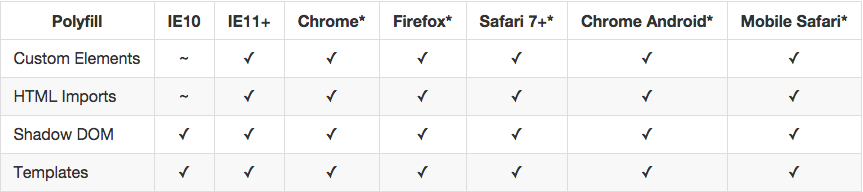
\includegraphics[width=1\linewidth]{images/chapter_tecnologie_abilitanti/tecnologie_abilitanti_polyfill.png}\hfill
 \caption[Supporto ai polyfill]{In tabella, le tecnologie web component supportate dai browser mediante uso di polyfill.}
 \label{fig:tecnologie_abilitanti_polyfill}
\end{figure}
Se il browser possiede gia un supporto nativo ai Web Component, webcomponents.js lo individua automaticamente e di conseguenza cambia modalità a favore del supporto nativo, in modo da garantire le migliori prestazioni possibili per il browser. 
Anche se molti sviluppatori sfruttano tutte le tecnologie offerte da webcomponents.js, il plugin è strutturato in modo da poter usare anche un sottoinsieme delle tecnologie offerte. 
I polyfills che webcomponents.js offre sono:
\begin{itemize}
\item Per quanto riguarda le tecnologie Web Components:
\begin{itemize} 
\item Custom Elements
\item HTML Imports
\item Shadow DOM
\end{itemize}
\item Per quanto riguarda il DOM:
\begin{itemize}
\item WeakMap (struttura dati più efficiente contro la perdita di dati in memoria)
\item Mutation Observers (per ascoltare i cambiamenti all’interno del DOM)
\end{itemize}
\end{itemize}
Le tecnologie di Web Component espongono delle API a basso livello; creare nuovi elementi HTML utilizzando direttamente le primitive offerte da queste tecnologie può richiedere una grande mole di lavoro da parte dello sviluppatore. Per questo motivo sono state create diverse librerie che semplificano lo sviluppo di nuovi componenti HTML: tra queste si fa menzione di X-Tag, Polymer e Bosonic. Fondamentalmente queste librerie fanno uso di strumenti di alto livello per ridurre la duplicazione del codice e rendere più semplice la creazione di nuovi componenti. Di base, tutte queste librerie utilizzano lo stesso Web Component polyfill. Sia Polymer che Bosonic offrono anche una libreria di web components pronti per essere utilizzati, e l’utilizzatore di questi componenti non dovrà preoccuparsi di quali librerie sono state usate per crearli. 
Delle tre librerie menzionate Polymer è quella più diffusa; nel paragrafo \ref{sec:chapter_tecnologie_abilitanti_polymer} vedremo come, mediante Polymer, sono stati sfruttati gli standard Web Components per la realizzazione dell’editor.

\subsection{Polymer}
\label{sec:chapter_tecnologie_abilitanti_polymer}
Come già accennato nel paragrafo precedente, polymer è una libreria studiata per rendere semplice e veloce la creazione di nuovi componenti HTML. Essa poggia sugli standard Web Components, e offre un insieme di funzionalità volte a ridurre la quantità di codice scritto, e a semplificare la creazione di elementi HTML complessi; inoltre, la libreria offre un catalogo di elementi già pronti per essere importati nelle applicazioni web. 
\\
\begin{figure}[htb]
 \centering
 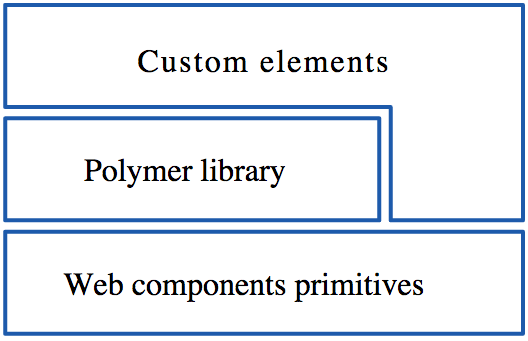
\includegraphics[width=0.5\linewidth]{images/chapter_tecnologie_abilitanti/tecnologie_abilitanti_polymer_stack.png}\hfill
 \caption[Strato Polymer]{In foto, la posizione dello strato Polymer rispetto alle tecnologie web components.}
 \label{fig:tecnologie_abilitanti_polymer_stack}
\end{figure}

Siccome il supporto nativo ai Web Components ancora non è presente in tutti i browsers, Polymer utilizza i polyfills di webcomponent.js. Con i polyfills, Polymer è compatibile con i seguenti browsers:
\\
\begin{figure}[htb]
 \centering
 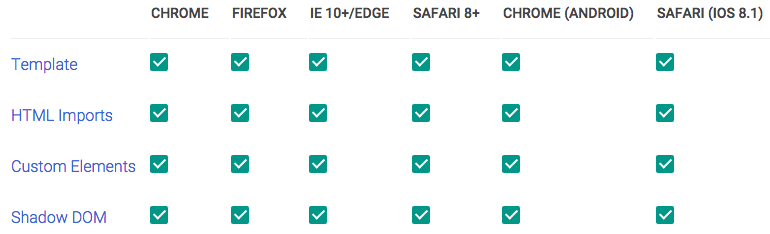
\includegraphics[width=1\linewidth]{images/chapter_tecnologie_abilitanti/tecnologie_abilitanti_poly_comp.png}\hfill
 \caption[Polymer e browser compatibili]{Compatibilità di polymer con i principali browser.}
 \label{fig:tecnologie_abilitanti_poly_comp}
\end{figure}
A questo punto verranno mostrate le principali funzionalità offerte da Polymer per la creazione di elementi HTML:
//
Per registrare un nuovo elemento nel browser si usa la funzione Polymer. La registrazione, di cui  prevede l’associazione di un tag riconoscitivo dell’elemento ad un prototipo, nel quale poter aggiungere metodi e proprietà all’elemento. La funzione Polymer prende come argomento un oggetto che definisce il prototipo dell’elemento, e restituisce un costruttore che può essere usato per istanziare l’elemento.
Inoltre la funzione definisce la catena prototipale per il nuovo elemento, collegandolo al prototipo base di Polymer, da cui eredita le funzioni in esso definite; questo esula lo sviluppare dal dover definire egli stesso una catena prototipale.
Il protitopo deve avere la proprietà is che specifica il tag HTML del nuovo elemento creato. Attualmente Polymer supporta l’estensione solamente di elementi HTML nativi, come \texttt{<input>} o \texttt{<button>}. Per estendere un elemento HTML nativo si inserisce nel prototipo la proprietà extends associata al tag dell’elemento che si vuole estendere. 
\begin{lstlisting}[language=HTML5, label={poly_code1}]
<script>
 //registro un nuovo elemento chiamato Custom Element
 Polymer({
  is: "custom-element",
  extends: 'input',
  factoryImpl: function(param) {
   this.param = param;
  },
  //lifecycle callback
  ready: function() {},
  created: function() {},
  attached: function() {},
  detached: function() {},
  attributeChanged: function(name, type) {}
 });
<\script>
\end{lstlisting}
Il metodo polymer restituisce un costruttore che viene usato per istanziare il nuovo custom element. Se si desidera passare degli argomenti al costruttore, bisogna specificare nel prototipo la funzione \texttt{factoryImpl}; ad esempio il custom element realizzato in \ref{poly_code1} può essere istanziato in in questo modo:
\begin{lstlisting}[language=JavaScript]
var el = new CustomElement('someproperty');
\end{lstlisting}
Un’altra funzionalità offerta la Polymer è implementazione nel prototipo base delle lifecycle callbacks secondo lo standard Custom Elements; le funzioni sono state rinominate e sono le seguenti:
\begin{itemize}
\item \texttt{created}, che corrisponde a createdCallback.
\item \texttt{attached}, che corrisponde a attachedCallback.
\item \texttt{detached}, che corrisponde a detachedCallback.
\item \texttt{attributeChanged}, che corrisponde a attributeChangedCallback.
\end{itemize}
Ovviamente è possibile utiizzare anche i metodi originali, implementandoli nel prototipo dell’elemento. Polymer aggiunge un’ulteriore callback, \texttt{ready}, che viene invocata quando Polymer ha terminato la creazione e l’inizializzazione di tutti i nodi interni al local DOM dell’elemento; infatti molti elementi possono includere all’interno dei nodi che implementano UI e comportamento dell’elemento: Polymer definisce questi nodi local DOM.
Per specificare il DOM da usare come local DOM dell’elemento, si usa l’elemento \texttt{<dom-module>}, a cui si assegna l’attributo id che coincide con la proprietà is del prototipo del nuovo elemento. All’interno del \texttt{<dom-module>} si inserisce un elemento \texttt{<template>}, e Polymer automaticamente copierà il contenuto del template nel local DOM dell’elemento.
\begin{lstlisting}[language=HTML5,label={code_poly2}]
<dom-module id="custom-element">
 <template>
  <p>I am a DOM element, and this is my local DOM</p>
 </template>
 <script>
  Polymer({
   is: 'custom-element'
  });
 </script>
</dom-module>
\end{lstlisting}
Nell’esempio \ref{code_poly2} il local DOM è statico, dal momento che il suo unico nodo \texttt{<p>} ha per valore una stringa fissa. Tuttavia nella maggior parte dei casi è preferibile che il local DOM possa cambiare dinamicamente, e per questo scopo Polymer ha introdotto la funzionalità \textbf{data binding}. 
Data Binding è uno strumento per associare una proprietà di un custom element ad un attributo di un elemento contenuto nel suo local DOM. E’ possibile fare il binding su una proprietà del componente racchiudendo un riferimento alla proprietà tra doppie graffe ({{ }}). Il contenuto nelle parentesi verrà sostituito dal valore della proprietà il cui riferimento è contenuto nelle graffe. Nell’esempio è possibile vedere un binding tra la proprietà \texttt{owner} di \texttt{custom-element}, definita mediante il costrutto \texttt{properties} che verrà descritto a breve, e l’attributo \texttt{owner} dell’elemento del local DOM di \texttt{custom-element}. 
\begin{lstlisting}[language=HTML5]
<dom-module id="custom-element">
 <template>
  This is <b>{{owner}}</b> custom element.
 </template>
 <script>
  Polymer({
   is: 'custom-element',
   properties: {
    owner: {
     type: String,
     value: "Daniel"
    }
   }
  });
 </script>
</dom-module>
\end{lstlisting}
Il costrutto utilizzato per la definizione della proprietà owner fa parte di altra funzionalità offerta da Polymer: le \textbf{declared properties}. 
E’ possibile dichiarare delle proprietà di un custom element aggiungendole ad un oggetto properties nel prototipo del custom element. Ogni proprietà facente parte delle API pubbliche dell’elemento, andrebbe dichiarata nell’oggetto properties. Attraverso l’oggetto properties è inoltre possibile usufruire di un’altra funzionalità di Polymer, ovvero \textbf{Property Observation}. 
E’ possibile mettersi in ascolto dei cambiamenti di una proprietà di un custom element, inserendo all’interno di essa l’attributo observer e associandovi una funzione setter detta change handler; nel momento in cui la proprietà subisce un cambiamento, la change handler viene chiamata con il vecchio e nuovo valore come argomenti.
\begin{lstlisting}[language=HTML5]
Polymer({
 is: 'custom-element',
 properties: {
  prop: {
   type: Boolean,
   observer: '_propChanged'
  }
 },
 _propChanged: function(newValue, oldValue) {
  this.toggleClass('prop',newValue);
  this.highlight = true;
 }
});
\end{lstlisting}